\chapter{Desenvolvimento do Jogo}\label{ch:Desenvolvimento}

O processo de desenvolvimento de jogos digitais é uma tarefa que exige do(s) desenvolvedor(es) conhecimentos de programação. Um jogo para ser desenvolvido, deve ser escrito em uma determinada linguagem de programação, o que acaba por obrigar que o(s) desenvolver(es) do jogo tenha(m) conhecimento sobre esta linguagem. Embora existam linguagens de programação visual, o conhecimento sobre lógica de programação ainda é parte fundamental e essencial para o desenvolvimento de um jogo. 

Um jogo digital requer conhecimentos computacionais específicos para o seu desenvolvimento. Aspectos técnicos e metodológicos devem ser levados em consideração durante todo o ciclo de desenvolvimento de um jogo. A \autoref{sec:Engenharia} trás fundamentação teórica detalhada a respeito dos principais aspectos metodológicos que tangem o jogo desenvolvido pela presente pesquisa. Brevemente, informa-se que o jogo desenvolvido pelo corrente trabalho acadêmico, segue a metodologia para o desenvolvido de jogos denominada de \ac{GAMED} \cite{aslan2016digital}. 

Definir uma metodologia de desenvolvimento é essencial para se gerenciar melhor os prazos e recursos necessários de um projeto. Dada a importância dessa etapa, é crucial que a escolha da mesma esteja devidamente fundamentada. Por tal razão, que a metodologia escolhida para guiar essa pesquisa é descrita no Capítulo de Fundamentação do presente trabalho acadêmico. Sendo assim, resta ao presente Capítulo, apresentar demais aspectos importantes que tange o jogo educacional desenvolvido pela corrente pesquisa. No entanto, é essencial salientar aqui que, embora aspectos artísticos, sonoros, ergonômicos e jurídicos sejam importantes no desenvolvimento de jogos, eles não são abordados neste trabalho, assim como questões sobre usabilidade, acessibilidade, escalabilidade, flexibilidade, criptografia e segurança de dados.

Aspectos de menor interesse científico e acadêmico encontram-se descritos detalhadamente no \ac{GDD} do jogo (\autoref{chap:DIE}). O \ac{GDD} é um documento que busca trazer maiores esclarecimentos sobre um determinado jogo. O documento pode conter desde as informações mais básicas de um jogo, até informações mais detalhadas de cunho técnico relacionadas ao seu desenvolvimento \cite{motta2013short}. Dito isso, o \ac{GDD} do jogo desenvolvido pela corrente pesquisa contempla ambos os casos, trazendo tanto informações de caráter mais básico, quanto informações de caráter mais detalhado.

O presente Capítulo apresenta as características gerais do jogo desenvolvido. Nesse sentido, tanto aspectos computacionais, quanto aspectos pedagógicos e metodológicos de ensino são descritos. Sendo assim, a \autoref{sec:motor} descreve as principais caraterísticas gerais que tangem o jogo desenvolvido por essa pesquisa, listando aspectos técnicos, tais como, dinâmicas e mecânicas utilizadas no jogo. A forma como essas mecânicas e dinâmicas interagem com os conceitos didáticos do jogo é descrita na \autoref{sec:DN}. Por fim, \autoref{sec:fim} dá as considerações finais do presente Capítulo. 

%-------------------------------------------------------------------------------------------------------------------

\section{Características Gerais}\label{sec:motor}

A presente pesquisa realiza o desenvolvimento de um \acf{JS}. O jogo em questão, baseia-se nas ideias propostas por \citeonline{diocesano2018infancia}. Visando apresentar as principais características que definem o \ac{JS} produzido, confeccionou-se um \ac{GDC}. A \autoref{fig:canvas} ilustra o \acl{GDC} do jogo elaborado pelo atual trabalho acadêmico. 

\begin{figure}[hbt!]
  \caption{\label{fig:canvas}\textit{Game Design Canvas}}\vspace{-0.2cm}
  \begin{center}
    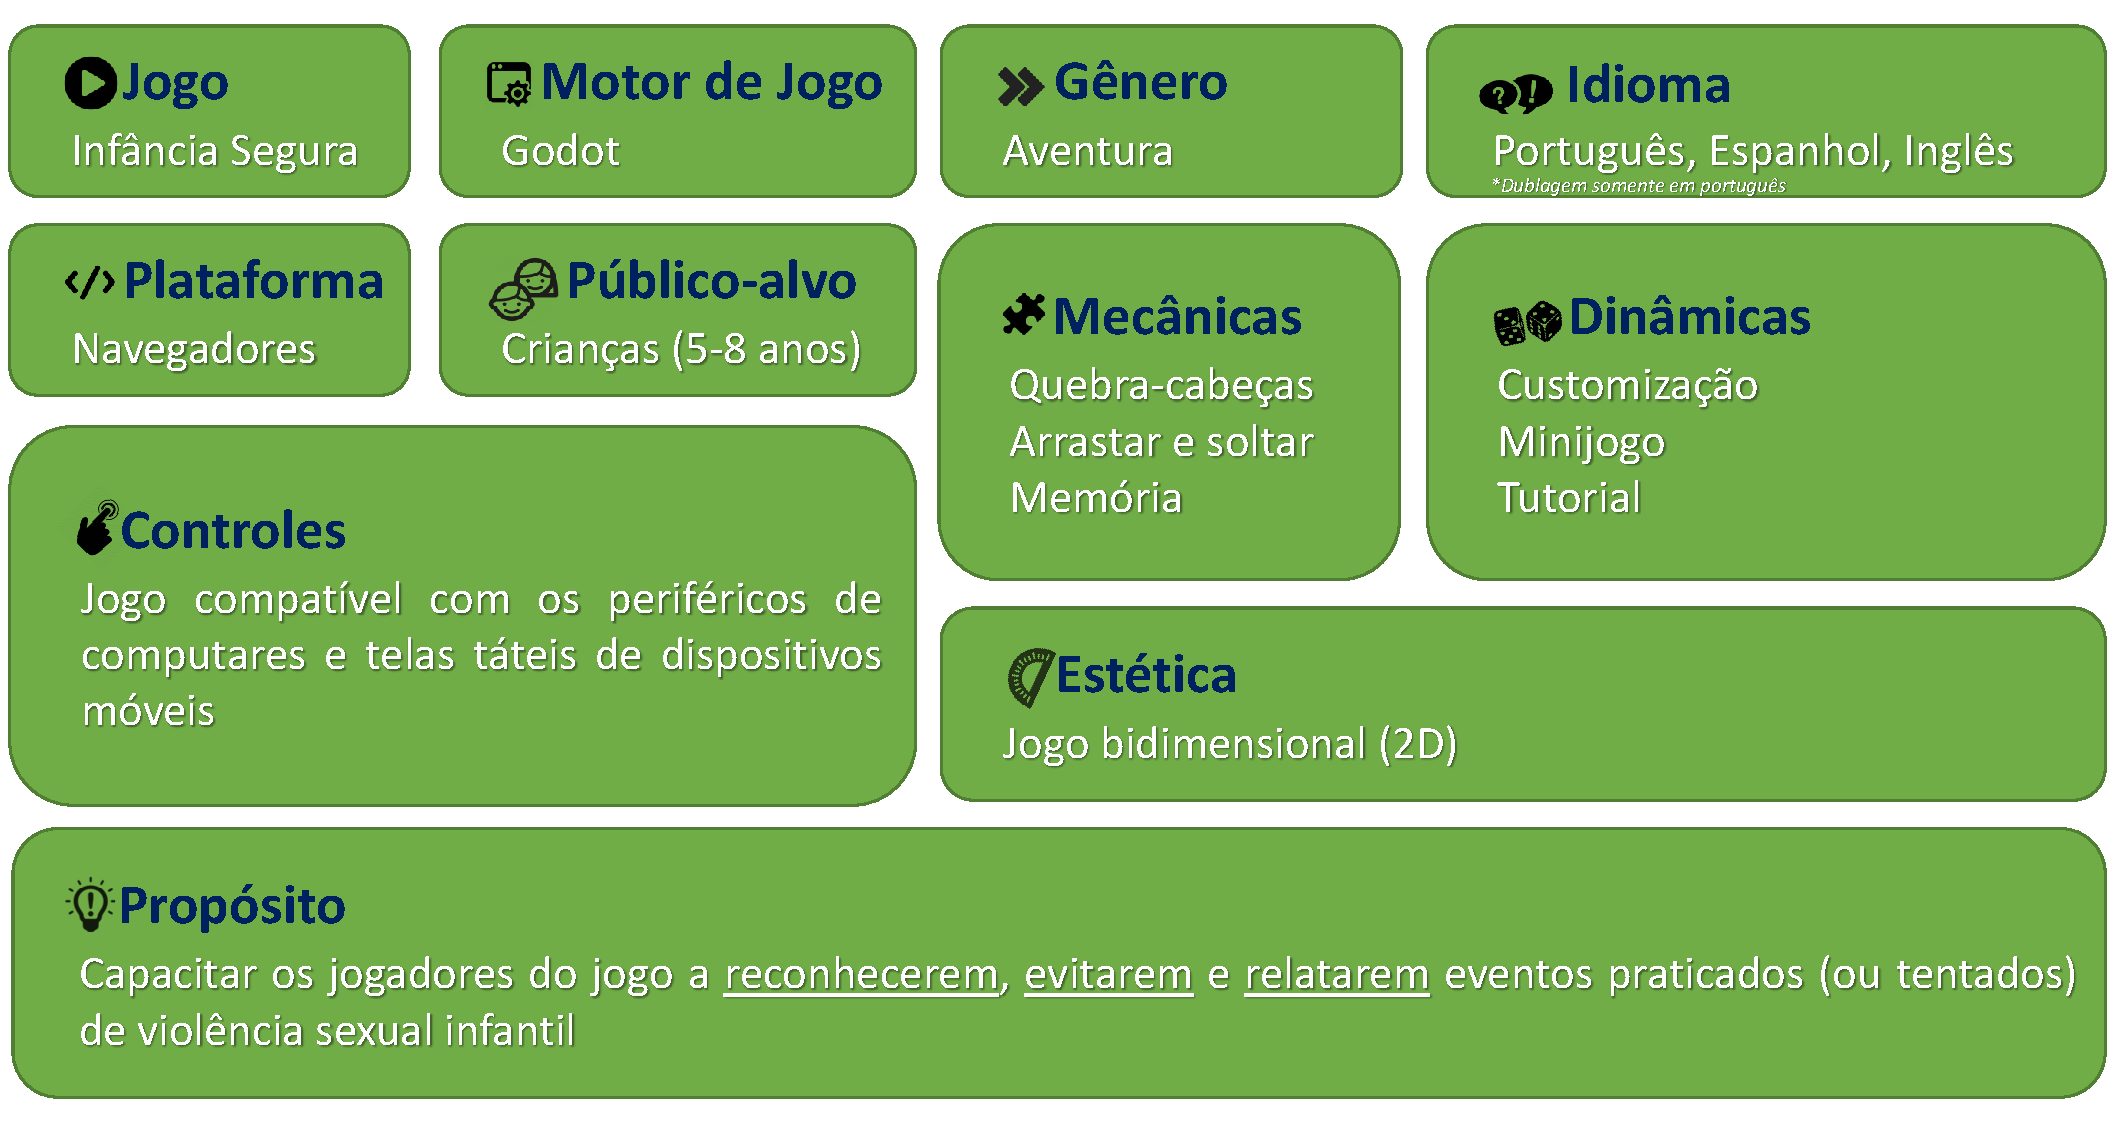
\includegraphics[width=\linewidth]{./Visuais/canvas2.pdf}
    \end{center}\vspace{-0.4cm}
  \legend{Fonte: Elaborada pelo autor (2021).}
\end{figure}

%A \autoref{fig:canvas} define as principais características do jogo desenvolvido. O jogo confecionado pelo correte trabalho herda algumas ideias propostas por \citeonline{diocesano2018infancia}, enquanto descarta outras (\textit{e.g.} o jogo original baseia-se em um dinâmica linear de exploração, ao invés de uma dinâmica de mundo aberto). Dentre os principais legados do jogo original estão: o nome do jogo, seu propósito, público-alvo e plataforma. O jogo denomina-se \textbf{Infância Segura}. Seu propósito consiste em desenvolver e aprimorar habilidades e conhecimentos específicos que viabilizem aos jogadores reconhecerem, evitarem e relatarem episódios praticados (ou tentados) de violência sexual infantil. Para atingir a classe infantil, definiu-se um público-alvo de crianças entre 5 (cinco) e 8 (oito) anos de idade. Essa idade é estabelecida com base nos conteúdos pedagógicos abordados pelo jogo, sendo conteúdos adequados a essa faixa etária de acordo com as orientações técnicas internacionais de educação em sexualidade da \citeonline{unesco2018international}. Buscando atingir um maior número de crianças, escolheu-se portar o jogo para navegadores, o que proporciona que o jogo esteja disponível a uma variedade maior de dispositivos com o mínimo de alterações ou adaptações no código-fonte \cite{carrara2018criancca}. Essa escolha, faz com que os controles do jogo sejam compatíveis aos periféricos dos computadores e as telas táteis dos dispositivos móveis.

A \autoref{fig:canvas} define as principais características do jogo desenvolvido. O jogo confecionado pelo correte trabalho herda algumas ideias propostas por \citeonline{diocesano2018infancia}, enquanto descarta outras (\textit{e.g.} o jogo original baseia-se em um dinâmica linear de exploração, ao invés de uma dinâmica de minijogos). Dentre os principais legados do jogo original estão: o nome do jogo, seu propósito, público-alvo e plataforma. O jogo denomina-se \textbf{Infância Segura}. Seu propósito consiste em desenvolver e aprimorar habilidades e conhecimentos específicos que viabilizem aos jogadores reconhecerem, evitarem e relatarem episódios praticados (ou tentados) de violência sexual infantil. Para atingir a classe infantil, definiu-se um público-alvo de crianças entre 5 (cinco) e 8 (oito) anos de idade. Essa idade é estabelecida com base nos conteúdos pedagógicos abordados pelo jogo, sendo conteúdos adequados a essa faixa etária de acordo com as orientações técnicas internacionais de educação em sexualidade da \citeonline{unesco2018international}. Buscando atingir um maior número de crianças, escolheu-se portar o jogo para navegadores, o que proporciona que o jogo esteja disponível a uma variedade maior de dispositivos com o mínimo de alterações ou adaptações no código-fonte \cite{carrara2018criancca}. Essa escolha, faz com que os controles do jogo sejam compatíveis aos periféricos dos computadores e as telas táteis dos dispositivos móveis.

%O jogo desenvolvido é de estética inteiramente bidimensional (2D) com perspectiva axonométrica. A bidimensionalidade do jogo agiliza o processo de desenvolvimento. A remoção uma dimensão do jogo, simplifica as etapas de programação e elaboração de cenários. Entretanto, jogos bidimensionais tendem a limitar a locomoção do personagem do jogador justamente por removerem uma dimensão. Para contornar isso, surgem os jogos em perspectiva axonométrica. Jogo axométricos, são jogos bidimensionais que não limitam a movimentação do jogador, permitindo que o mesmo possa locomover seu personagem tridimensionalmente em todo o cenário do jogo. 

O jogo desenvolvido é de estética inteiramente bidimensional (2D). A bidimensionalidade do jogo agiliza o processo de desenvolvimento. A remoção uma dimensão do jogo, simplifica as etapas de programação e elaboração de cenários. Para que o cenário e todos os demais aspectos do jogo sejam mais compreensíveis ao jogador é essencial promover um sistema de tutoria. Um sistema de tutoria auxilia o processo de compreensão das regras e da estrutura do jogo ao jogador. O esclarecimento sobre as regras e sobre a estrutura do jogo pode ser feito tanto por um tutor, quanto por um sistema de tutorial. A utilização de um sistema de tutorial substitui a necessidade de um tutor \cite{buchinger2014sherlock}. Um sistema de tutorial consite na ideia de  ensinar ao jogador como funcionam as dinâmicas de um jogo, apresentando as regras e as ações que o jogador pode exercer. Existem diversos meios para ensinar isso ao jogador. No caso do jogo desenvolvido, o sistema de tutorial utilizado segue uma estrutura simples, na qual uma certa solução inicial de uma determinada fase é apresentada ao jogador. Tal estrutura se baseia na capacidade de abstração do jogador em compreender que a solução inicial apresentada pode ser associada e replicada para as demais soluções existentes em uma determinada fase. Compreendendo os princícios básicos de uma solução, o jogador então é capaz de usar esse conhecimentos para alcançar êxito nas demais soluções de uma certa fase. 

%baseia-se na ideia de um tutor virtual que acompanha o jogador durante todo o jogo. O tutor virtual acompanha o personagem do jogador sem se distanciar muito. Isso é feito para reforçar os ensinamentos de que uma criança deve estar sempre acompanhada, além disso. %espera-se que tal funcionalidade traga um sentimento de companheirismo ao jogador. 
%Junto a este sistema de ajuda ao jogador, também é implementado a dinâmica do herói mudo. %ou dinâmica do protagonista silencioso.

%A dinâmica do herói mudo (ou protagonista silencioso) permite que o jogador tenha uma maior imersão no jogo. Nessa dinâmica, o personagem do jogador não se expressa de maneira verbal \cite{domsch2017dialogue}. Graças a isso, não há o risco do personagem do jogador se utilizar de palavras ou de elementos contextuais que o jogador desconheça, proporcionando assim, uma conexão maior entre personagem e jogador. Como artifício, para dar enredo a história do jogo, as frases são transferidas para um personagem que o jogador não possui controle (o personagem tutor), com o intuito de evitar assim, uma disrupção da interligação entre personagem e jogador. Embora o personagem do jogador não fale; todos os diálogos do jogo são transcritos textualmente e verbalmente. A depender da configuração do jogo, os diálogos podem ser exibidos em português, espanhol, ou inglês. No entanto, a verbalização dos dialógicos (localização), encontra-se disponível somente em português. A localização associada ao texto escrito proporciona acessibilidade do jogo as crianças (falantes de português) que não se encontram plenamente alfabetizadas \cite{limeira2015avaliaccao}. 

Para ajudar ainda mais o jogador, todos os diálogos do jogo são transcritos textualmente e verbalmente. A depender da configuração do jogo, os diálogos podem ser exibidos em português, espanhol, ou inglês. No entanto, a verbalização dos dialógicos (localização), encontra-se disponível somente em português. A localização associada ao texto escrito proporciona acessibilidade do jogo as crianças (falantes de português) que não se encontram plenamente alfabetizadas \cite{limeira2015avaliaccao}. 

Com o intuito de facilitar a leitura dos textos, todos os diálogos transcritos obedecem recomendações tipográficas para materiais didáticos infantis \cite{lourenco2011tipografia}. Em outras palavras, o jogo desenvolvido se utiliza e se apoia em caracteres classificados como infantis, ou seja, caracteres que se aproximam mais da escrita manual em comparação com a escrita digital (\textit{e.g.} `a' em caracter adulto, `\textit{a}' em caracter infantil).

O jogo para prevenção da violência sexual infantil projetado neste trabalho é do gênero aventura. Os jogos de aventura são jogos em que o jogador assume o papel de um protagonista em uma história interativa com exploração e resolução de quebra-cabeças. Os quebra-cabeças do presente jogo se traduzem em minijogos voltados a prevenção da violência sexual infantil. Ao se tratar do público infantil, observou-se que o gênero aventura, se destaca como o gênero de jogo que mais agrada de forma igualitária, meninos e meninas \cite{brandtzaeg2009children}. 

Os minijogos do jogo desenvolvido pela corrente pesquisa utilizam alguns elementos da cultura popular. A utilização de elementos da cultura popular no ensino é capaz aumentar os níveis de motivação e compreensão dos alunos \cite{giroux1988schooling, cheung2001use, duncan2004your, chik2011learner}. Desta forma, o jogo desenvolvido se apoia em alguns componentes da cultura popular com o intuito de melhor engajar seu público-alvo, deixando os assuntos ministrados mais interessantes e atraentes. 

Para o desenvolvimento e produção de um jogo digital, existem majoritária dois caminhos. Um jogo digital pode ser produzido em uma linguagem de programação, seguindo os protocolos e estruturas específicas de um determinado dispositivo, ou pode ser produzido sob um motor de jogo (\textit{Game Engine}). Motor de jogo é o nome dado a qualquer plataforma voltada para o desenvolvimento de jogos. Os motores de jogos proporcionam um ambiente completo para a criação de jogos, com toda a parte gráfica e sonora já abstraídas. Isso permite ao(s) desenvolvedor(es) exportar o jogo para diferentes sistemas computacionais realizando alterações mínimas no código-fonte \cite{bishop1998designing, machado2009serious}.

Existem vários motores voltados para o desenvolvimento de jogos. O motor optado por este trabalho é o \textit{Godot}\footnote{\textit{Godot} é um motor de jogos totalmente gratuito de código aberto sob a licença permissiva do MIT (CC BY 3.0). O motor pode ser adquirido por meio do seguinte endereço: \url{https://godotengine.org/}.} (versão 3.3). Em comparação aos demais motores de jogos, o \textit{Godot} se destaca por ser totalmente gratuito, adaptado ao idioma português e por exportar os jogos para múltiplos sistemas \cite{scherer2020analise}. Salienta-se que a última versão estável da plataforma \textit{Godot} é a versão 3.3 (lançada no dia 21 abril de 2021). Por tal razão essa é a versão que fundamenta as bases e o andamento do corrente trabalho acadêmico. Sendo utilizada a versão para \textit{Windows} 10. O ambiente de desenvolvimento do jogo assenta-se então, basicamente no sistema operacional \textit{Windows} 10 \textit{Education}. As configurações de desenvolvimento são um processador Intel(R) Core(TM) i7-8750H, 16 \acsu{GB} de memória RAM DDR4 e placa de vídeo GeForce GTX 1060. O ambiente de testes é realizado sob essas mesmas especificações, mas também em um \textit{tablet} da \textit{Multilaser} M10A, com processador Quad Core 1.3 \acsu{GHz}, 2 \acsu{GB} de memória RAM e sistema operacional \textit{Android} 8.1. Salienta-se que o \textit{tablet} utilizado para testes durante o desenvolvimento do jogo é o mesmo utilizado na etapa de testes com usuários da atual pesquisa (\autoref{ch:Avaliacao}).

Por fim, embora a plataforma \textit{Godot} exporte seus jogos para múltiplos sistemas, é importante destacar que o jogo desenvolvido neste trabalho está exportado apenas para navegadores. Fica a cargo de pesquisa futuras a adaptação do código-fonte para portar o jogo para diferentes sistemas operacionais, possibilitando assim, que o jogo possa ser baixado e executado sem necessidade de uma conexão constante com os servidores. Em adendo, salienta-se que a atual versão do jogo grava dados de seus jogadores em um banco de dados. O registro dos dados dos jogadores é uma herança do jogo original proposto por \citeonline{diocesano2018infancia}. Salienta-se no entanto, que os dados não são filtrados ou tratados, sendo acessíveis somente através de requisições ao servidor. Ou seja, o corrente trabalho não implemente uma ferramenta amigável para acesso dos dados dos jogadores, como proposto originalmente por \citeonline{diocesano2018infancia}. A presente pesquisa se dispõe, apenas, no desenvolvimento do jogo em si, e sua validação. Cabe então a pesquisas futuras, a confecção de uma plataforma mais agradável de acesso a essas informações, fornecendo visualização mais clara e precisa no que diz respeito ao desempenho dos jogadores, a professores ou responsáveis.  


%-------------------------------------------------------------------------------------------------------------------

\section{Desenho de Níveis e Ensinamentos}\label{sec:DN}

O \acf{JS} desenvolvido ministra assuntos sensíveis relacionados a sexualidade e a prevenção da violência sexual infantil. Por tal razão, todo o fundamental teórico do jogo advém de documentos devidamente revisados por especialistas na área de educação e sexualidade \cite{unesco2018international}. Ainda no aspecto pedagógico, salienta-se que o jogo não se utiliza de elementos visualmente realistas. Ou seja, o jogo não se utiliza de artes realistas para apresentar um determinado conceito ou uma determinada situação. A literatura relata que a utilização de imagens reais de cunho sexual trazêm desconforto para alguns indivíduos, por tal razão toda a arte utilizada no jogo assume o estilo de um cartum \cite{albert2020desenvolvimento}.

O \ac{JS} desta pesquisa possui uma estrutura metodológica de ensino baseada em quatro princípios a serem ministrados: Anatomia (\autoref{subsec:1}), Direitos (\autoref{subsec:2}), Denúncias (\autoref{subsec:3}) e Redes Sociais (\autoref{subsec:4}). Cada um desses princípios se traduz em uma fase no jogo, cada qual composta de três níveis. A \autoref{fig:conceitos} apresenta cada fase do jogo associada aos seus respectivos níveis.

\begin{figure}[hbt!]
  \caption{\label{fig:conceitos}Conceitos abordados}\vspace{-0.3cm}
  \begin{center}
    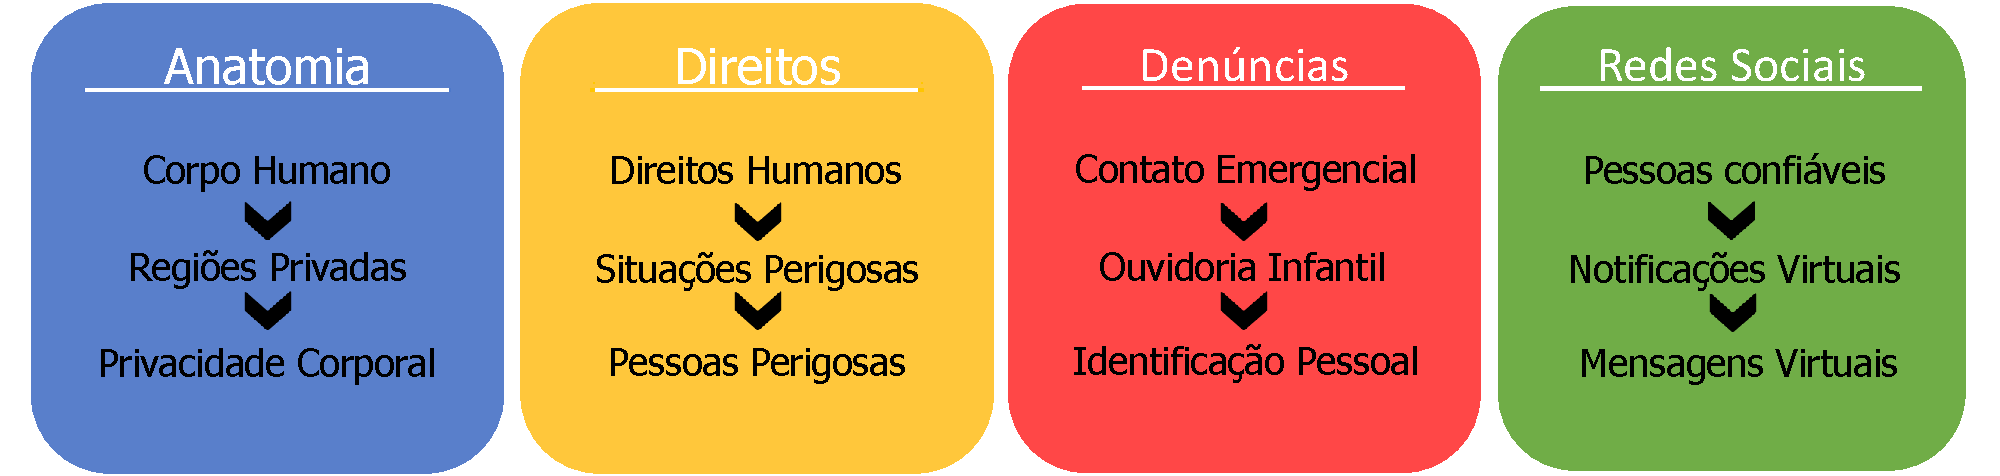
\includegraphics[width=\linewidth]{./Visuais/EsquemaFases2.pdf}
    \end{center}\vspace{-0.3cm}
  \legend{Fonte: Elaborada pelo autor (2021).}
\end{figure}

\vspace{-0.4cm}

A \autoref{fig:conceitos} ilustra de maneira resumida cada um dos conteúdos a serem ministrados pelo jogo. Cada conteúdo é ministrado em um cenários específico no jogo e por um personagem específico. O jogador é livre para intercambiar entre os cenários sem quaisquer prejuízos, podendo alternar entre as fases da maneira que melhor lhe convir. Respectivamente, os conceitos sobre anatomia são ministrados em um cenário que simula um \textbf{Hospital}. Os direitos das crianças são ensinados em um cenário que simula uma \textbf{Escola}. A realização de denúncias é um assunto ensinado em um cenário que simula uma \textbf{Delegacia}. E a proteção no ambiente virtual das redes é ministrado em cenário que simula um \textbf{Cibercafé}.

A jogabilidade de jogo é flexível, permitindo ao jogador intercambiar entre as fases sem qualquer punição. Entretanto, os níveis das fases obedecem a uma linearidade tanto de enredo, quando pedagógica (\textit{e.g.} na fase da anatomia o jogador deve necessariamente aprender antes sobre os nomes das partes do corpo, para em seguida aprender quais são as partes íntimas do corpo, para por fim aprender os locais onde as pessoas podem tocar no corpo). O jogador tem liberdade para abandonar um nível sempre que desejar. Contudo, os últimos níveis são alcançáveis apenas após a conclusão dos anteriores. 

%-------------------------------------------------------------------------------------------------------------------

\subsection{Anatomia}\label{subsec:1}

O jogo desenvolvido ministra conteúdos relacionados a anatomia humana em um ambiente hospitalar. Três minijogos buscam ensinar ao jogador questões sobre o \textbf{Corpo Humano}, \textbf{Regiões Privadas} e \textbf{Privacidade Corporal}. A \autoref{fig:Hospitalzinho} ilustra as dinâmicas utilizadas em cada um dos minijogos. Todos os conceitos abordados por cada um destes minijogos são ministrados por um personagem que representa um médico. 

\begin{wrapfigure}[26]{r}{6.0cm}%pulando 26 linhas
  \vspace{-20pt}
  \caption{\label{fig:Hospitalzinho}Hospital}
  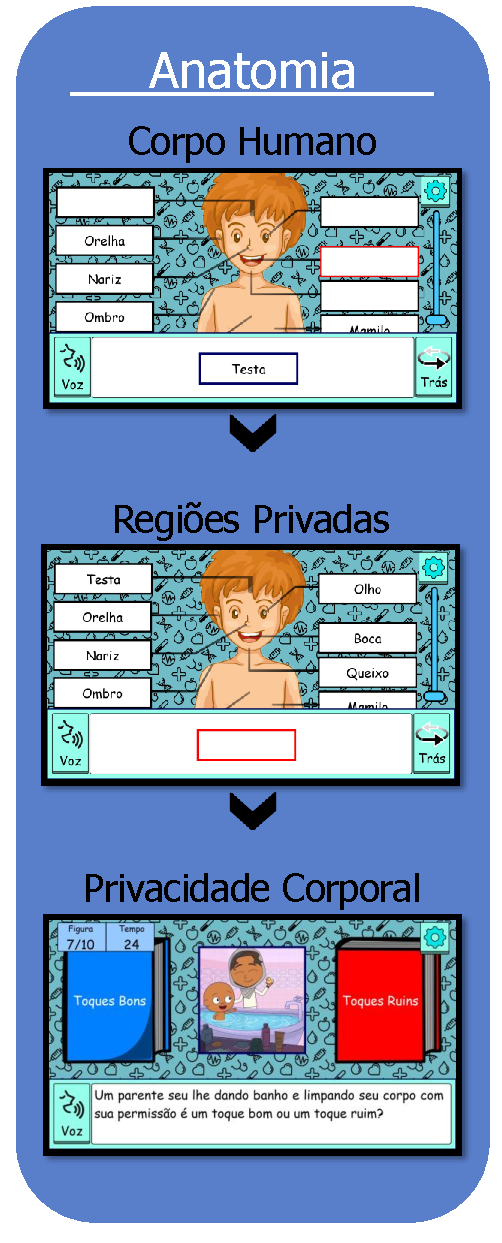
\includegraphics[width=\linewidth]{./Visuais/Hospital2.pdf}
  \vspace{-1.0cm}
  \legend{Fonte: Elaborada pelo autor (2021).}
\end{wrapfigure}

O primeiro minijogo (\textbf{Corpo Humano}) busca ensinar ao jogador o nome correto das partes do corpo. Com o auxílio de um mural ilustrativo, o jogador é capaz reconhecer as nomenclaturas corretas do corpo humano masculino e feminino. %Após um determinado evento, as  algumas peças do mural caem. 
O jogador deve nesse jogo demonstrar seus conhecimentos sobre o corpo humano, inserindo as peças em suas respectivas posições. As peças vão aparecendo uma a uma no centro da caixa de diálogo, sendo que o jogador deve arrastá-las e movê-las para suas posições originais. Peças colocadas em posições válidas notificam o jogador por meio se um sinal sonoro de acerto. Peças colocadas em posições inválidas emitem um aviso de erro ao jogador de forma sonora e visual. 

O segundo minijogo (\textbf{Regiões Privadas}) busca ensinar ao jogador as partes íntimas do corpo humano. O personagem do médico educa o jogador sobre as zonas privadas e não privadas do corpo, utilizando como apoio o mesmo mural do primeiro minijogo. As regiões privadas são representadas por peças com contorno vermelho no mural. Após o jogador ter adquirido esse conhecimento no tutorial, o jogo se inicia sem as peças destacadas em vermelho. Neste momento o jogador deve demonstrar suas habilidades de memorização levando os contornos vermelhos para as peças que representam as partes íntimas. A notificação de acertos e erros ao jogador ocorre da mesma maneira que no primeiro minijogo. %Peças inseridas em posições incorretas emitem sonoramente e visualmente um aviso de erro ao jogador. Peças em posições válidas emitem apenas um sinal sorono de acerto.

O terceiro minijogo (\textbf{Privacidade Corporal}) busca ensinar ao jogador sobre toques bons e ruins. Neste minijogo são apresentados dois livros, um apenas com imagens de toques bons e outro apenas com imagens de toque ruins. %Um dado evento faz com que as imagens se misturem entre os livros. 
O jogador deve demonstrar seus conhecimentos classificando devidamente as imagens. As imagens vão aparecendo uma por uma na caixa de diálogo, com o jogador tendo que movê-las para seus respectivos livros. A conclusão deste minijogo encerra a etapa de anatomia. %Após esse minijogo, o jogador completa a etapa de anatomia do jogo. 

%-------------------------------------------------------------------------------------------------------------------

\subsection{Direitos}\label{subsec:2}

O jogo projetado neste trabalho se propõe a ensinar o jogador sobre seus direitos e deveres em um cenário escolar. Três minijogos buscam ensinar ao jogador questões sobre \textbf{Direitos Humanos}, \textbf{Situações Perigosas} e \textbf{Pessoas Perigosas}. A \autoref{fig:Escola} ilustra as dinâmicas utilizadas em cada um dos minijogos. Todos os conceitos abordados são ministrados por um personagem que representa uma professora. 

\begin{wrapfigure}[26]{r}{6.0cm}%pulando 26 linhas
  \vspace{-20pt}
  \caption{\label{fig:Escola}Escola}
  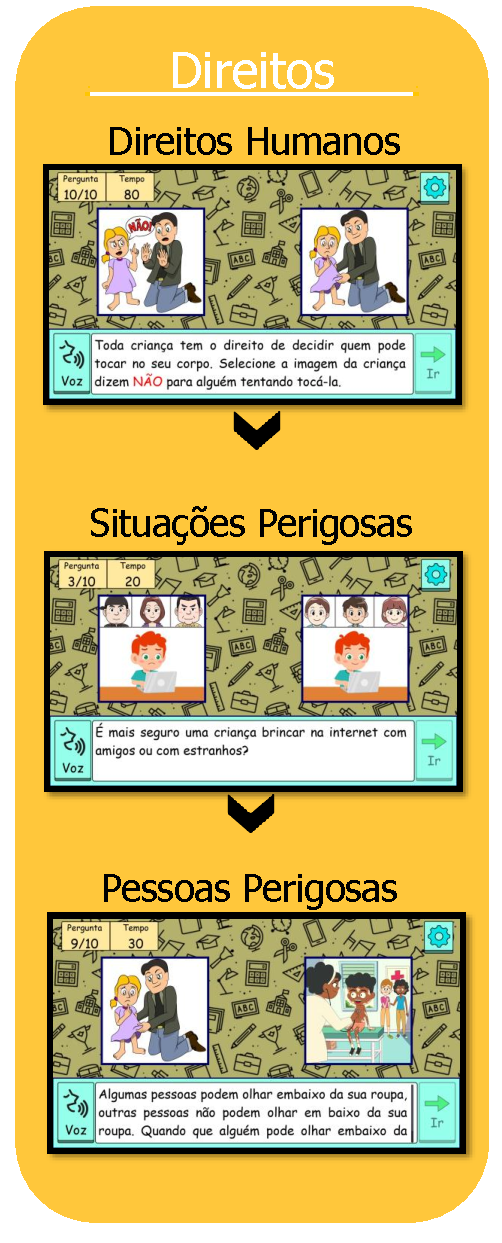
\includegraphics[width=\linewidth]{./Visuais/Escola2.pdf}
  \vspace{-1.0cm}
  \legend{Fonte: Elaborada pelo autor (2021).}
\end{wrapfigure}

O primeiro minijogo (\textbf{Direitos Humanos}) busca ensinar ao jogador sobre os direitos da criança no Brasil e no mundo. O minijogo discorre sobre os direitos e deveres das crianças. Por meio de um jogo de perguntas e respostas com imagens o jogador deve associar determinado direito ou dever com uma das imagens apresentadas. O jogador então, além de ser ensinado verbalmente e textualmente sobre seus direitos, demonstra seus conhecimentos em uma representação visual. Tal método de ensino, demonstra a capacidade de abstração do jogador ao criar uma imagem mental dos conceitos aprendidos e associar essa imagem mental a uma imagem no jogo. O jogador é gratificado sonoramente por seus acertos. Quaisquer erros cometidos pelo jogador são justificados em uma mensagem sonora possibilitando que o jogador compreenda seus equívocos. 

O segundo minijogo (\textbf{Situações Perigosas}) visa educar o jogador sobre sua segurança. O jogador é ensinado que as crianças não estão totalmente protegidas de seus direitos, sendo importante tomar cuidado com determinadas situações que podem colocá-las em risco. %na qual os direitos das crianças seriam desrespeitados. 
Com o auxílio de imagens, um conjunto de situações é apresentado ao jogador onde o jogador deve optar em escolher duas situações. Nesse jogo de perguntas e respostas o jogador deve então demonstrar sua perspicácia em evitar situações potencialmente perigosas. A notificação de acertos e erros ocorre de forma igual ao primeiro minijogo.

O terceiro minijogo (\textbf{Pessoas Perigosas}) busca ensinar ao jogador sobre pessoas que podem desrespeitar os direitos das crianças. O minijogo em si realiza uma série de perguntas e respostas similar as do segundo minijogo, porém ao invés de apresentar situações, pessoas são apresentadas. Nesse minijogo, o jogador deve então demonstrar sua habilidade evitando pessoas que apresentem atitudes potencialmente perigosas. Após a conclusão deste minijogo, o jogador finaliza a etapa de direitos. 

%-------------------------------------------------------------------------------------------------------------------

\subsection{Denúncias}\label{subsec:3}

O \ac{JS} desenvolvido apresenta ao jogador algumas formas nas quais são possíveis formalizar uma denúncia. Três minijogos buscam ensinar ao jogador questões relacionadas a \textbf{Contato Emergencial}, \textbf{Ouvidoria Infantil} e \textbf{Identificação Pessoal}. A \autoref{fig:DelegaciaDP} ilustra as dinâmicas utilizadas em cada um dos minijogos. Os conceitos desse ambiente são passados por um personagem de um delegado. 

\begin{wrapfigure}[26]{r}{6.0cm}%pulando 26 linhas
  \vspace{-20pt}
  \caption{\label{fig:DelegaciaDP}Delegacia}
  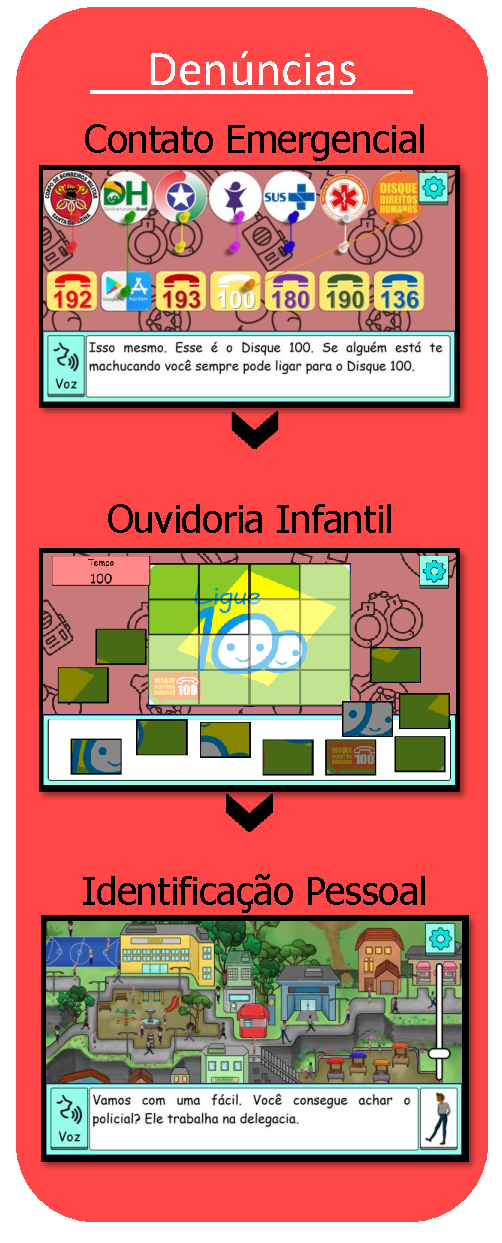
\includegraphics[width=\linewidth]{./Visuais/Delegacia2.pdf}
  \vspace{-1.0cm}
  \legend{Fonte: Elaborada pelo autor (2021).}
\end{wrapfigure}


O primeiro minijogo (\textbf{Contato Emergencial}) busca apresentar ao jogador os principais telefones de emergência do Brasil. Para isso, o minijogo em questão introduz um conjunto de números telefônicos e logotipos. Nesse jogo, o jogador é instruído a associar corretamente, por intermédio de pinos, os números telefônicos e seus respectivos serviços (logotipos). Associações erradas emitem um sinal sonoro e visual ao jogador, com o pino retornando para a sua posição inicial. Associações corretas, emitem uma mensagem de acerto ao jogador, a qual explica sobre o número telefônico e sobre em quais situações tal serviço deve ser utilizado. Ao mesmo tempo, o pino se fixa ao número telefônico, não retornando a sua posição inicial.

%O primeiro minijogo (\textbf{Contato Emergencial}) busca apresentar ao jogador as formas virtuais de se realizar uma denúncia no Brasil. Para isso, o minijogo em questão introduz um computador onde um jogo de datilografia se inicia. Nesse jogo, o jogador é instruído a pesquisar e digitar corretamente os canais nacionais de denúncia. O jogo obedece uma estruturo lúdico-pedagógica de forma a ser acessível para o jogador que não encontram-se totalmente alfabetizado, acendendo as letras que devem ser selecionadas pelo jogador. Letras não acesas, selecionadas pelo jogador, não manifestam resposta (sendo um sistema de notificação de erro menos intrusivo), travando o progresso do jogador até que uma letra acesa seja selecionada. 

O segundo minijogo (\textbf{Ouvidoria Infantil}) ensina ao jogador sobre as linhas telefônicas para a denúncia de crimes contra a criança. Um mural com um número telefônico é apresentado ao jogador. %Após o jogador visualizar o mural, um dado evento, faz com que o mural se fragmente. 
Em um jogo de quebra-cabeça o jogador deve então montar o mural. A dinâmica lúdica utilizada neste jogo, prolonga o contato do jogador com o canal de denúncia do Disque 100, ampliando assim a retenção da informação. Peças colocadas em posições incorretas não provocam sinais sonoros e nem provocam sinais visuais de erro ao jogador (as peças simplesmente não se fixando no mural). Entretanto, peças colocadas em locais corretos ficam fixadas ao mural, impossibilitando de serem movidas novamente. 

%O terceiro minijogo (\textbf{Identificação Pessoal}) busca ensinar ao jogador como realizar denúncias pessoalmente e como interagir com pessoas. Neste minijogo, um livro ilustrado é apresentado ao jogador. As situações ilustradas representam eventos ordenados. Uma dada situação faz com que a ordem das ilustrações seja embaralhada. Neste momento, o jogador é confrontado a montar novamente a ordem dos acontecimentos (eventos) ilustrada no livro. 
%O jogador então demonstra como se comportar em um conjunto de situações e como relatar os acontecimentos para uma pessoa confiável. 
%O término deste minijogo, implica na conclusão da etapa de denúncias. 

O terceiro minijogo (\textbf{Identificação Pessoal}) busca ensinar ao jogador como realizar denúncias pessoalmente e como interagir com pessoas. Neste minijogo, uma pequena cidade é apresentada ao jogador, repleta de indivíduos. O jogador deve então procurar por certos indivíduos nessa cidade. Sempre que um determinado indivíduo é encontrado, uma mensagem é apresentado ao jogador, explicando sobre como interagir com determinado indivíduo, devendo manter distância ou não. O término deste minijogo, implica na conclusão da etapa de denúncias. 

%-------------------------------------------------------------------------------------------------------------------

\subsection{Redes Sociais}\label{subsec:4}

O jogo desenvolvido pela corrente pesquisa elenca, ao jogador, maneiras seguras para se proteger na \textit{internet}. Três minijogos buscam ensinar ao jogador questões sobre \textbf{Pessoas Confiáveis}, \textbf{Notificações Virtuais} e \textbf{Mensagens Virtuais}. A \autoref{fig:Cibercafe} ilustra as dinâmicas utilizadas em cada um dos minijogos. Todos os conceitos abordados por cada um destes minijogos são ministrados por um personagem de um robô. 

\begin{wrapfigure}[26]{r}{6.0cm}%pulando 26 linhas
  \vspace{-20pt}
  \caption{\label{fig:Cibercafe}Cibercafé}
  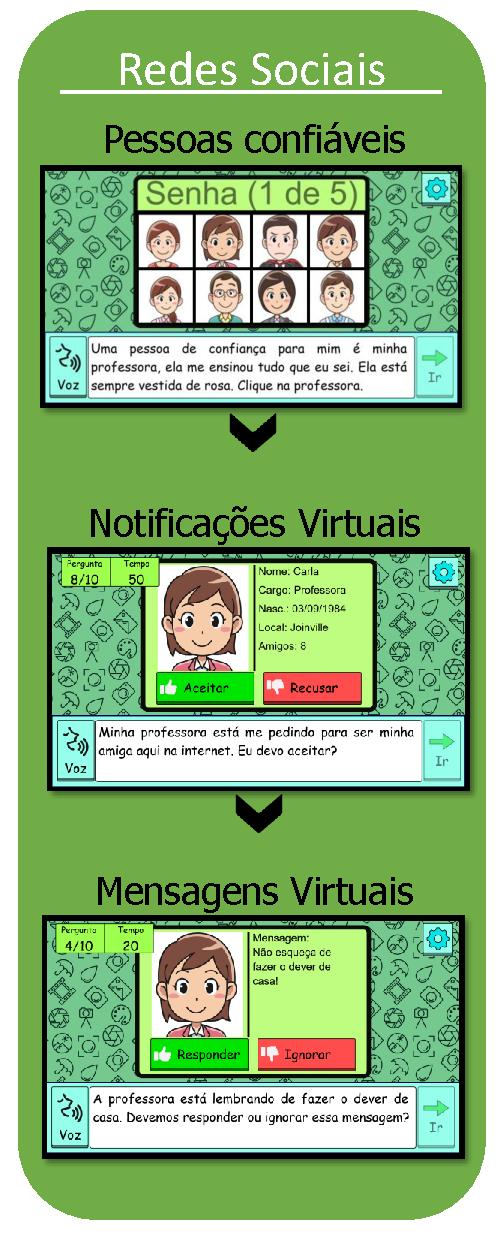
\includegraphics[width=\linewidth]{./Visuais/Cibercafe2.pdf}
  \vspace{-1.0cm}
  \legend{Fonte: Elaborada pelo autor (2021).}
\end{wrapfigure}

O primeiro minijogo (\textbf{Pessoas Confiáveis}) busca ajudar o jogador a identificar 5 (cinco) pessoas de confiança. A dinâmica deste minijogo consiste na tentativa e erro do jogador em montar um conjunto de pessoas de confiança até atingir uma combinação que esteja correta (imposta pelo minijogo). O minijogo associa as 5 (cinco) pessoas de confiança apresentadas, a outro personagem existente no jogo. Tal abordagem é tomada com o intuito de evitar associações diretas com parentes falecidos do jogador. Sendo assim, o minijogo em questão se propõe a ajudar o jogador a compreender de maneira mais genérica o que define uma pessoa confiável e o que define uma pessoa não confiável. 

%Salienta-se que minijogo evita relacionar diretamente as pessoas confiáveis (imposta pelo jogo) com pessoas reais que o jogador conheça, visando evitar associações com parentes falecidos do jogador. Sendo assim, o minijogo associa as pessoas confiáveis apresentadas a outro personagem no jogo. Durante esse minijogo as escolhas certa e erradas são justificadas ao jogador, ajudando-o a compreender o que define uma pessoa confiável e uma pessoa não confiável

O segundo minijogo (\textbf{Notificações Virtuais}) busca ensinar ao jogador como se comportar nas redes sociais. O minijogo enfatiza sobre os cuidados necessários para se acessar e se utilizar as redes sociais, salientando que algumas redes exigem uma idade mínima para sua utilização (\textit{e.g.} a rede social \textit{Facebook} define uma idade mínima de treze anos para seus usuários). A dinâmica deste minijogo consiste em ensinar ao jogador a adicionar apenas pessoas conhecidas, tendo sempre muito cuidado com a existência de perfis falsos se passando por pessoas conhecidas. O jogador precisa então, aceitar e recursar devidamente pedidos de amizade, além de aprender a desfazer amizades (caso um erro seja cometido). 

O terceiro minijogo (\textbf{Mensagens Virtuais}) ensina ao jogador como se comunicar na \textit{internet}. O minijogo se baseia no princípio que alguns serviços na \textit{internet} possibilitam o compartilhamento de mensagens sem a prévia autorização do indivíduo receptor (\textit{e.g.} o mensageiro instantâneo \textit{Whatsapp}). Desta forma, o minijogo se propõe a educar o jogador a não compartilhar informações com estranhos; relatando sempre tais acontecimentos para um adulto de confiança. Após esse minijogo, o jogador completa a etapa de Redes Sociais. 

%-------------------------------------------------------------------------------------------------------------------

\section{Considerações Finais}\label{sec:fim}

O \acf{JS} projetado por este trabalho é constituído por 12 (doze) minijogos voltados a educar crianças sobre questões relacionadas a prevenção da violência sexual infantil. A maioria dos minijogos, apresentam a mesma Barra de Estado (em inglês: \acl{HUD}), como pode ser observado nas telas do jogo das Figuras \ref{fig:Hospitalzinho}, \ref{fig:Escola}, \ref{fig:DelegaciaDP} e \ref{fig:Cibercafe}. A Barra de Estado, é uma região da tela do jogador na qual informações ou elementos são dispostos de modo a não atrapalhar e nem obstruir a visão do jogador, sendo anexados normalmente nas extremidades da tela na qual o jogo está sendo executado. %Os elementos da Barra de Estado do jogo desenvolvido são: um botão para silenciar/desilenciar o jogo (canto superior direito), um botão para congelar/descongelar o jogo e um botão vermelho para sair dos minijogos (centro superior). O botão vermelho situado na região superior de todos os 12 (doze) minijogos é um botão presente apenas nestes momentos. Quando o jogador está transitando entre os cenários do jogo, o botão não é apresentado. Salienta-se que um jogador só é livre para acessar e transitar livremente no jogo, após um breve cadastro. 

Os elementos da Barra de Estado do jogo desenvolvido são: um sistema de pontuação, situado no canto superior esquerdo (de alguns níveis) e uma pequena engrenagem, situada no canto superior direito (de todos os níveis). O sistema de pontuação é omitido em alguns níveis com o intuito de evitar uma maior poluição visual (\textit{e.g.} na terceira fase da Delegacia, o sistema de pontuação ocultaria a visão do jogador no que diz respeito a cidade apresentada). No entanto, salienta-se que, todos os níveis (com ou sem sistema de pontuação aparente) pontuam o tempo utilizado pelo jogador para a sua conclusão. Outros níveis, além de pontuarem o tempo, pontuam também a quantidade de erros cometidos pelo jogador. 

O jogo não apresentad a quantidade de erros cometidos pelo jogador no sistema de pontuação, sendo só apresentado a ``pergunta corrente'' relativa a quantidade total de perguntas. Esse artifício é utilizado por duas razões. A primeira razão, é a de evitar o constragimento do jogador, ao fixar seus erros cometidos na tela. A segunda razão, é a de deixar claro ao jogador quantas perguntas ainda devem ser respondidas, evitando assim qualquer forma de angústica relacionada ao desconhecimento sobre número de perguntas restantes para se alcançar a conclusão de um determiando nível.

O jogo desenvolvimento pelo atual trabalho exige o preenchimento de um cadastro. Neste cadastro são requisitadas duas informações: o gênero do jogador e uma credêncial de acesso. Nos níveis sobre \textbf{Anatomia} (\autoref{subsec:1}) o jogador aprende sobre as nomeclaturas e as regiões privadas do corpo humano relacionadas ao gênero gênero que informou ao jogo. O gênero do jogador é requisitado para fornecer uma abordagem de ensino mais voltada ao indivíduo. A credêncial de acesso permite que uma determinada criança seja associada a um identificador, tal identificador se mantém em todas as etapas da corrente pesquisa. Desta forma é possível associar o desempenho de um determinado jogador no jogo e seu desempenho nas demais etapas deste trabalho. Isso tudo, sem que a devida identidade da criança tenha que ser revelada, garantindo assim seu anonimato. 

Ao final de cada nível, um relatório geral sobre o desempenho do jogador é apresentado. Nele, o jogador é capaz de identificar sua quantidade de erros e o tempo utilizada para a conclusão do nível. O jogador é convidado então a rejogar o jogo e superar seu desempenho, comentendo menos erros em um menor tempo. Salienta-se que demais informação geradas pelo sistema não são apresentados ao jogador em nenhum momento (\textit{e.g.} ações erradas executadas pelo jogador). 

As informações coletadas pelo jogo servem para compreender melhor o desempenho de cada jogador e suas preferências, além de identificar eventuais dificuldades que um determinado jogador possa estar enfrentanto, proporcionando assim uma a aprendizagem mais voltada ao indivíduo, e não, ao coletivo \cite{carrara2018criancca}. Além disso, é possível identificar também, eventuais falhas conceituais ou estruturais no jogo (\textit{e.g.} caso vários jogadores manifestem o mesmo erro em um dado momento do jogo, isso pode indicar três problemas principais: ou a ação requisitada pelo jogador pode ser muito difícil e descalibrada para a sua idade; ou o sistema de pontuação do jogo pode estar classificando uma determinada ação correta como uma ação errônea; ou a ação é mal formulada sendo confusa e ambigua para o jogador).

O jogo opera unicamente em navegadores, necessitando de uma conexão via servidor para ser carregado no navegador. A conexão via servidor ainda se faz necessária durante os minijogos, pois é durante estes momentos que o jogo realiza requisições ao banco de dados. Visando garantir a integridade das informações; o sistema envia seus registros ao banco de dados em dois momentos. Em um momento inicial, cada ação realizada pelo jogador gera uma requisição ao banco de banco de dados, o qual armazena a ação do jogador. Em um segundo momento, ao final de um nível, o sistema envia novamente, porém em bloco, o total de ações realizada pelo jogador naquele nível, podendo assim se verificar a consitência das informações no banco de dados. 

Os minijogos do jogo desenvolvido possuem seus ensinamentos baseados orientações técnicas internacionais de educação em sexualidade \cite{unesco2018international}. Os únicos dois minijogos que não encontram-se em harmonia com as orientações internacionais são os conceitos de \textbf{Contato Emergencial} e \textbf{Ouvidoria Infantil}. A introdução destes dois conceitos ao jogo, surge como uma medida de fortalecer as estratégias e campanhas nacionais de conscientização infantil. O estudo bibliográfico do presente trabalho identificou medidas nacionais focadas na divulgação dos ramais e canais de denúncia dos direitos das crianças. Almejando a divulgação de tais canais, optou-se em anexar, os dois conceitos citados, ao jogo. Com exceção destes conceitos, todos os demais assuntos estão em consonância com as orientações da \citeonline{unesco2018international}. 

Diante do exposto no presente Capítulo, enfatiza-se que o \ac{JS} desenvolvido por este trabalho baseia seus ensinamentos em conceitos didáticos reconhecidos na área em questão. Assim como, baseia seu processo de desenvolvimento em aspectos técnicos reconhecidos no campo de  desenvolvimento de jogos. O próximo passo da corrente pesquisa, consiste na realização de testes com usuários para se verificar a eficácia, ou não, do jogo no que tange o combate a violência sexual infantil. 